\chapter{Linear Cross Entropy}
\label{ch:lxe}
\epigraph{Check the circuit}{Spock to helmsman;
  \citefield{butlerCage1988}{booktitle}
--- \citefield{butlerCage1988}{number}}

PTIM: \cite{langEntanglementTransitionProjective2020}

Fisher/Altman PRL, hier wird die LXE definiert: \cite{liCrossEntropyBenchmark2023}

Nicolai: \enquote{Das ist eines der Paper, die Fisher zitiert, wo die LXE eingeführt wurde.} \cite{baoSymmetryEnrichedPhases2021}

arXiv:2306.00058, LXE fürs PTIM, preprint \cite{tikhanovskayaUniversalityCrossEntropy2023}

MIPT allgemein, hier leider eher weniger ahnung warum ich das in dieses Kapitel rein
gemacht hab zum zitieren. \cite{baoTheoryPhaseTransition2020}

Sampling stuff aus appendix von \cite{roserDecodingProjectiveTransverse2023}

In this chapter we examine a measure proposed by
\citeauthor{liCrossEntropyBenchmark2023} in \cite{liCrossEntropyBenchmark2023}
to circumvent the sampling problem. This measure is called the \emph{linear
cross entropy} (abbreviated as LXE). Although it is a novel quantity, its properties in hybrid
circuits, and general random circuits, have already been explored in varying
degrees of detail. Even for the projective transverse-field Ising model (PTIM),
a study has been conducted (cf. ref.
\cite{tikhanovskayaUniversalityCrossentropy$mathbbZ_2$2024}). In the present
chapter, we will investigate the properties of the linear cross entropy in
general and for the projective transverse-field Ising model. We will also
evaluate its quality as an order parameter for the phase transition of the
PTIM.

The chapter is structured as follows. We will first introduce the quantity
itself in \cref{sec:lxe-defn}, where we also provide a shortcut for computing
the LXE in clifford circuits. We then investigate the behavior of it in the
PTIM, comparing it to the entanglement entropy of an ancilla qubit attached to
the system. Next, we introduce faulty gates to the process and examine the LXE
for a system with errors. Lastly, we motivate the discarding of either $X$ or
$ZZ$ measurement results with probability-theoretic arguments and evaluate the
utility of the LXE for the different cases.

\section{Definition and properties}\label{sec:lxe-defn}
In this section we provide a definition for the linear cross entropy (LXE)
$\chi$ and a detailed derivation for its computation in Clifford circuits.

Hier Definition und die ganze algebra/mathematik. dann den part zu LXE in
stabilizer (mit dieser projection und so)

Auch verschiedene Trackings?

\subsection{General random circuits}
We first introduce the linear cross entropy (also abbreviated as LXE) in the
context of general random quantum circuits. We then provide a concrete
description and expression of the LXE for our system, the projective
transverse-field Ising model.

Consider a hybrid circuit with some cicruit layout $C$, consisting of unitary
and measurement gates. The measurement gates within the circuit yield results
$m_i$, which are collected in the sequence $\mathbf{m} = \{m_1, m_2, \ldots,
m_N\}$, where $N$ is the number of measurement gates. We call this sequence of
measurement outcomes the \emph{measurement record}. For some initial state
$\rho$ of our hybrid circuit, we can compute the \emph{unnormalized} output
state as
\begin{align}\label{eq:rho-m}
  \rho_\mathbf{m} \equiv C_\mathbf{m} \rho C^\dagger_\mathbf{m}
.\end{align}
Here, $C_\mathbf{m}$ is the time-ordered product of all gates in the circuit,
unitary and measurement, and can be written as
\begin{align}
  C_\mathbf{m} = 
.\end{align}
The action of $C_\mathbf{m}$ on the initial state
$\rho$ is the mathematical object representing one possible trajectory with
measurement outcomes $\mathbf{m}$. Leaving the state unnormalized after 
projection operations is a deliberate choice; it allows us to define the
probability of a certian measurement record.

\begin{defn}[Probability of a trajectory]\label{defn:prob-traj}
  Given a random circuit $C$ and an initial state $\rho$ with corresponding
  measurement record $\mathbf{m}$, the probability of $\mathbf{m}$ is denoted
  by
  \begin{align}
    P\left( \mathbf{m} \mid C, \rho \right) \equiv \Tr[\rho_\mathbf{m}] =
    \Tr[C_\mathbf{m} \rho C^\dagger_\mathbf{m}]
  .\end{align}
\end{defn}

Although we do not want to delve too deep into probability theory at this point,
let us nonetheless first convince ourselves that \cref{defn:prob-traj} really does
define a proper probability measure. To this end, consider the simplest example of
a circuit with initial state $\rho = \dyad{+}$ and a single measurement in the
Pauli-$Z$ basis. By \cref{eq:rho-m} our unnormalized output state reads
\begin{align}\label{eq:prob-example}
  \rho_\mathbf{m} = \mathbb{P}_m \dyad{+} \mathbb{P}_m^\dagger = \begin{cases}
    \frac{1}{2}\dyad{0}, & m = 1 \\
    \frac{1}{2}\dyad{1}, & m = -1
  \end{cases}
\end{align}
with $\mathbb{P}_m = \frac{1}{2}\left(\mathds{1} + m Z \right)$. Computing the
trace then yields $\frac{1}{2}$ for the probability of each trajectory. This is
also consistent with our expectation from elementary quantum mechanics. As
projectors sum to the identity (completeness), all the probabilities sum to
$1$, as they should.
Furthermore, since unitaries leave the norm invariant, the trace only picks up
projections. However, one needs to be careful here. Applying a Hadamard gate to
$\dyad{+}$ transforms the state, and the probabilities change.\footnote{The
  probabilities for the outcomes of a Pauli-$Z$ measurement become $1$ and
$0$}. Conversely,
applying a Hadamard gate to any of the output states in \cref{eq:prob-example}
does not alter the trace, but rather the output state itself.

We will later continue this discussion for the measurement-only circuit of the
PTIM. For now, we employ \cref{defn:prob-traj} and define the circuit-level
linear cross entropy $\chi_C\left(\rho, \sigma  \right)$.

\begin{defn}[Linear cross entropy]\label{defn:lxe}
  Given a random circuit $C$ with two distinct initial states $\rho$ and
  $\sigma$, and measurement records $\mathbf{m}$, the normalized linear cross
  entropy is defined as
  \begin{align}\label{eq:lxe-c-defn}
    \chi_C = \sum_{\mathbf{m}} P(\mathbf{m} \mid C, \rho) \frac{P(\mathbf{m} \mid
      C, \sigma)}{\sum_{\mathbf{m}'}\left(P(\mathbf{m}' \mid
      C, \sigma)\right)^2}
  ,\end{align}
  where the sums $\sum_\mathbf{m}$ go over all possible measurement outcomes of
  the measurement gates in the circuit.
\end{defn}
Most times when dealing with random circuits, we want to investigate numerous
different circuit realizations for a given parameter (usually probability).
Hence, when referring to the linear cross entropy, we will mostly refer to the
circuit-averaged linear cross entropy,
\begin{align}
  \chi \equiv \expval{\chi_C}_C
.\end{align}
We will later also see the utility of defining $\chi$ and $\chi_C$ this way,
especially concerning the denominator in \cref{eq:lxe-c-defn}. For now it
suffices to remark that it is a normalizing factor such that the linear cross
entropy is bounded from above by 1, $0 \leq \chi \leq 1$.

We can interpret this quantity like a classical fidelity between two
probability distributions. For two given initial states, we have a probability
distribution over measurement records. For each measurement record,
\cref{defn:prob-traj} provides a way to quantify the probability. For these
probabilities, the linear cross entropy quantifies the overlap of one
probability distribution with the other. If $\chi = 1$, the probability
distributions are identical, and if we chose different initial states, a unit
linear cross entropy tells us that this circuit (or parameter $p$) is not
suited to distinguish between the initial states $\rho$ and $\sigma$. On the
other hand, if $\chi=0$, we have no measurement record, which is compatible
with $\rho$ and $\sigma$ simultaneously.

\subsection{Clifford circuits and PTIM}\label{sec:lxe-for-ptim}
Now that we have introduced the general concept of the linear cross entropy and
defined the relevant quantities formally, we will examine it more closely in
the context of the projective transverse-field Ising model. As we are able to
simulate the PTIM with a stabilizer simulator, we will also introduce a way to
compute the LXE in Clifford circuits, which will be implemented in the
simulator.

In \cref{eq:lxe-c-defn}, the choice of placement of the individual
probabilities is a deliberate one. It is to highlight the fact that we are
averaging a quantity depending on $\sigma$ over a probability distribution that
depends on $\rho$. As a means of cirumventing the sampling problem, we'd like
$\sigma$ to correspond to a classical simulator and $\rho$ to the experiment.
It will therefore prove useful to examine the part dependent on $\sigma$ more
closely, as it will later enable us to efficiently. 
As intermediate step we first derive an
expression for the probabilities $P\left( \mathbf{m} \mid C, \rho \right)$,
laid out in \cref{lem:prob-traj-cliff}.
\begin{lem}[Probability of a trajectory in measurement-only Clifford circuits]\label{lem:prob-traj-cliff}
  Given a Clifford circuit $C$ with $N$ measurement gates and no other gates, with initial
  stabilizer state $\rho$, the probability of a measurement record is
  \begin{align}
    P\left(\mathbf{m} \mid C, \rho\right) = 2^{-N_\mathrm{rand}}
  ,\end{align}
  where $N_\mathrm{rand} \leq N$ is the number of random outcomes for the
  measurement gates.
\end{lem}

\begin{proof}
Suppose we have a Clifford circuit $C$ with $N$ measurement gates and an
$n$-qubit initial stabilizer state $\rho$. We already
know from \cref{sec:stab-basics} that there are two types of measurement
outcomes, random or deterministic. Each measurement potentially has 2 outcomes,
and in the former case each outcome has probability $1 / 2$ of occuring. (The
other outcomes, the deterministic ones, trivially have unit probability.)
Furthermore, we know that $\rho$ can be expressed as the product of projectors
\begin{align}
  \rho = \frac{1}{2^n} \prod_{i=1}^n (I + g_i)
\end{align}
or equivalently as a sum of all stabilizer group elements
\begin{align}
  \rho = \frac{1}{2^n} \sum_{g\in \mathrm{Stab}(\rho)} g
.\end{align}

If we now subject $\rho$ to the circuit $C$, we obtain a measurement record
$\mathbf{m}$. By \cref{defn:prob-traj} we compute the probability by tracing the
unnormalized output state (cf. \cref{eq:rho-m}), which in turn is obtained by application
of the respective projectors on the input state, i.e.
\begin{align}
  \rho_\mathbf{m} = C_\mathbf{m}\ \rho \ C_\mathbf{m}^\dagger 
  = T\left\{\prod_i^N\mathbb{P_i}\right\}\ \rho \ T\left\{\prod_i^N\mathbb{P_i}\right\}^\dagger 
.\end{align}
Here, $T\{\bullet\}$ is the time-ordering operator and $\mathbb{P}_i$ is the
projection operator on measurement outcome $i$. The probability of some
measurement record is then given by
\begin{align}
  P\left(\mathbf{m} \mid C, \rho\right) = \Tr[C_\mathbf{m} \rho
  C_\mathbf{m}^\dagger]
,\end{align}
which can be written as
\begin{align}
  P\left(\mathbf{m} \mid C, \rho\right) = \Tr[T\left\{\prod_i^N
  \mathbb{P}_i\right\}\rho]
,\end{align}
with the cyclic property of the trace and $\mathbb{P}^2 = \mathbb{P}$.
We can now consider the successive application of measurement gates.
We know that each of the $N$ measurements is either random or deterministic.
Let us therefore consider these two cases separately.
\par{Case 1 -- Deterministic outcome:}
If a measurement has a deterministic outcome, the measurement operator was
already part of the stabilizer group. We can therefore construct a set of
commuting operators $\langle g_i\rangle$, containing the measurement operator
$M$, which generate the
stabilizer group. If we let $g_1=M$ w.l.o.g., we have
\begin{align}
  P\left(\mathbf{m} \mid C, \rho\right) 
  &= \Tr[ \mathbb{P}_N \cdots \mathbb{P}_i \rho ] \nonumber\\
  &= \frac{1}{2^{n-1}}\Tr[\mathbb{P}_N \cdots \frac{1}{2} (I + M)\frac{1}{2} (I + g_1)
  \prod_{i=2}^n (I + g_i)] \nonumber\\
  &= \frac{1}{2^{n-1}}\Tr[\mathbb{P}_N\cdots \frac{1}{2}(I+M) \prod_{i=2}^n (I+g_i)] \nonumber\\
  &= \frac{1}{2^n}\TR[\mathbb{P}_N\cdots \mathbb{P}_{i+1} \prod_{i=1}^n
  (I+g_i)] \label{eq:prob-determ}
,\end{align}
where we used the fact that $\mathbb{P}^2 =\mathbb{P}$. The last line of
\cref{eq:prob-determ} tells us that deterministic measurements do nothing on
the state and the probability.
\par{Case 2 -- Random outcome:}
In the case of a random outcome, the operator to be measured was not in the
stabilizer group. Technically, it should be replaced, which is done by
conjugation with the projector. However, it turns out that for the probability,
we only need to consider a single projection. It is
\begin{align}
  P\left(\mathbf{m} \mid C, \rho\right) 
  &= \Tr[ \mathbb{P}_N \cdots \mathbb{P}_i \frac{1}{2^n}\sum_{g \in
  \mathrm{Stab}(\rho)} g]\nonumber\\
  &= \Tr[ \mathbb{P}_N \cdots \frac{1}{2} \left(\frac{1}{2^n} \sum_{g \in
  \mathrm{Stab}(\rho)} g + \sum_{g \in \mathrm{Stab}(\rho)} Mg\right) ]
.\end{align}
Since the second sum is exclusively one over Pauli matrices, which are traceless,
they don't contribute to the total. We thus have
\begin{align}
  P\left(\mathbf{m} \mid C, \rho\right) 
  = \Tr[\mathbb{P}_N \cdots \mathbb{P}_{i+1} \frac{1}{2^{n+1}}
  \sum_{g\in\mathrm{Stab}(\rho)} g]
.\end{align}

Combining cases 1 and 2, knowing that measurements with deterministic outcomes
don't alter the state at all, we have
\begin{align}
  P\left(\mathbf{m} \mid C, \rho\right) 
  &= \Tr[\frac{1}{2^{n+N_\mathrm{rand}}} \sum_{g\in\mathrm{Stab}(\rho)}
  g]\nonumber\\
  &= \frac{1}{2^{N_\mathrm{rand}}} = 2^{-N_\mathrm{rand}}
.\end{align}
%
%that each of the $N$ measurements is either a projection onto a stabilizer of
%$\rho$ or an alteration of the state in one or another way with probability $1
%/2$. Thus, any projection onto a measurement with deterministic outcome will
%act as identity on $\rho$. Consequently, we are left with $N_\mathrm{rand}$
%random outcomes to measurements, each of them with probability $1/2$. 
\end{proof}

We can now use this result to find a nice expression for the linear cross
entropy in Clifford circuits, and in particular the projective transverse-field
Ising model.
\begin{thm}[LXE for Clifford circuits]\label{thm:lxe-cliff}
  Let $C$ be a Clifford circuit with $N$ measurement gates and a measurement
  record $\mathbf{m}$ obtained from a realization of $C$ with some initial
  state $\rho$. Furthermore, let
  $\sigma \neq \rho$ be a different state, where $\mathbf{m}'$ are all possible
  measurement records from applying $C$ on $\sigma$. Then
  \begin{align}\label{eq:diesesding}
      \frac{P(\mathbf{m} |
      C,\sigma)}{\sum_{\mathbf{m'}}\left(P(\mathbf{m}'|C,\sigma)\right)^2}
      = \begin{cases}
        1 & \qquad{\sigma\text{ is compatible with }C \text{ and }
        \mathbf{m}}\\
        0 & \qquad{\sigma\text{ is not compatible with }C \text{ and }
        \mathbf{m}}\\
      \end{cases}
  .\end{align}
\end{thm}

\begin{proof}
  We can consider two (disjoint) cases:
  \begin{enumerate}
    \item No projection in $C_\mathbf{m}$ is orthogonal to $\sigma$, meaning
      that $\sigma$ is compatible with $C$ and $\mathbf{m}$.

      This implies that the trace in the computation of $P\left(\mathbf{m} \mid
      C,\sigma\right)$ will always be strictly above $0$. In fact, the
      probability will be $2^{N_\mathrm{rand}}$, since each projection was
      successful. Together with the fact that there are $2^{N_\mathrm{rand}}$
      measurement gates we have
      \begin{align}
      \frac{P(\mathbf{m} |
      C,\sigma)}{\sum_{\mathbf{m'}}\left(P(\mathbf{m}'|C,\sigma)\right)^2} =
      \frac{2^{-N_\mathrm{rand}}}{\sum_{\mathbf{m}'} 2^{-2N_\mathrm{rand}}}
      = \frac{2^{-N_\mathrm{rand}}}{2^{-N_\mathrm{rand}}} = 1
      .\end{align}

    \item At least one projection in $C_\mathbf{m}$ is orthogonal to $\sigma$,
      meaning that $\sigma$ is not compatible with $C$ and $\mathbf{m}$.

      Here we have at least one projection in $C_\mathbf{m}$, which projects
      $\sigma$ onto the $0$-vector. Incidentally, we require \emph{exactly} one
      projection to be orthogonal, since we then have no object that can be
      projected to anything. Thus, the trace becomes $0$, and as a consequence
      we have
      \begin{align}
      \frac{P(\mathbf{m} |
      C,\sigma)}{\sum_{\mathbf{m'}}\left(P(\mathbf{m}'|C,\sigma)\right)^2} = 0
      .\end{align}
  \end{enumerate}
\end{proof}

The second case in the proof of \cref{thm:lxe-cliff} is an interesting one to
consider, especially in the context of the PTIM. Suppose we run a PTIM circuit
on some $n$-qubit platform with an initial state of $\ket{\phi_0} = \left( \ket{0\cdots 0} +
\ket{1\cdots 1} \right) / \sqrt{2}$ or $\rho = \dyad{\phi_0}$. This produces a measurement record, which we
then feed into a classical simulator with an orthogonal Bell state
$\ket{\varphi_0} = \left( \ket{0\cdots 0} - \ket{1\cdots 1} \right) / \sqrt{2}$
or $\sigma = \dyad{\varphi_0}$.
There are of course other orthogonal Bell states we could choose as initial
state for our simulator. However, these two states are additionally orthogonal
in the logical basis. That is, if we encode information in $\ket{\phi_0}$, the
opposite information is encoded in $\ket{\varphi_0}$. That this choice is a
reasonable one gets even more apparent when considering generating sets of the
respective stabilizers,
\begin{align}\label{eq:rhosigmagenerators-lxe}
  G_\rho = \langle X\ldots X, Z_1Z_2,\ldots,Z_{n-1}Z_n\rangle \quad{\text{and}}
  \quad
  G_\sigma = \langle -X\ldots X, Z_1Z_2,\ldots,Z_{n-1}Z_n\rangle
.\end{align}
Notice that they are almost identical with a different sign in front of the
global $X$ stabilizer, implying orthogonality in the logical basis. In the
hypothetical, measurement outcomes of $\rho$ are projected onto $\sigma$.
Let us consider the two types of measurement, pairwise $ZZ$ and single-site
$X$. Performing a pairwise $ZZ$ measurement is a stabilizer measurement,
apparent from the generating sets given in \cref{eq:rhosigmagenerators-lxe}. A
measurement thereof will (at least initially) produce deterministic measurement
outcomes with $m = +1$. This is different for the $X$ measurements. Initially,
an $X$ measurement will not have an outcome we can infer beforehand. This,
however, is the case for both of them, up to a certain degree, since the
pairwise $Z$ stabilizers anticommute with the single-site $X$ measurement. This
also provides an explanation on why this is not always the case. If $X$
measurements are sufficiently frequent, there will be a point where there are
no $ZZ$ generators left, as all of them were replaced by $X$ by means of
measuring. Consequently, subsequent measurements of $X$ are deterministic,
which will detect the sign difference of the global $X$ stabilizer. This
detection would correspond to the point where the initial cluster dies in the
colored cluster model.

It turns out that this is the only case for the circuit-level linear cross
entropy to be $0$, i.e. $\chi_C = 0$. One can argue from the structure of the
stabilizer group, or just the generating set, that any measurements producing a
random outcome will produce a random outcome no matter what the previous
results were.\footnote{They are \enquote{Markovian} in that sense.} For an
outcome to be random, the measurement operator may not be contained in the
stabilizer of the state. Conversely, for an outcome to be deterministic, the
operator is a stabilizer. After measuring, the operator is guaranteed to be in
the stabilizer group of the state and subsequent measurements of this operator
produce the same result with unit probability. With the structure of the group
changed, we also have new anticommuting measurement operators, and so on. This
boils down to the conclusion that once the circuit $C$ is fixed, the
\emph{type} of measurement outcome is fixed. One could tell, without knowing
the actual outcomes to measurements, which of them were random and which were
deterministic. As such, a given circuit, which detects the sign difference
between $\sigma$ and $\rho$, does so in all of the runs, as deterministic
measurement outcomes stay so regardless of the previous history. Consequently,
the circuit-level linear cross entropy is $0$ regardless of measurement record
$\mathbf{m}$, if $C$ contains a deterministic measurement in $X$, where the
outcome is not given by a previous measurement, but by the sign of the initial
global $X$ stabilizer.

%We will henceforth refer to this mechanism of
%the linear cross entropy going to $0$ as mechanism \textsf{A}. As a
%visualization of this mechanism, confer with \cref{fig:mechanism-a}, showing a
%minimal example of a circuit detecting the sign difference.
\Cref{fig:mechanism-a} shows a minimal example of vanishing linear cross
entropy on the circuit level with initial states chosen as orthogonal Bell
states.

\begin{figure}[t]
  \centering
  \begin{tikzpicture}
  % Vertical separation between rho and sigma
  \draw[black,very thick] (5,0) -- (5,6.5);

  \node [init] at (2.5,.4) (rho) {$\rho$ (Experiment)\\$S = \langle
  +XX, ZZ\rangle$};
    %\\ $S_\rho = \langle X\ldots X,Z_1Z_2,
    %\ldots, Z_{n-1}Z_n\rangle$};
  \node [init] at (7.5,.4) (sigma) {$\sigma$ (Simulation)\\$S = \langle
  -XX,ZZ \rangle$};
    %\\ $S_\rho = \langle X\ldots X,Z_1Z_2,
    %\ldots, Z_{n-1}Z_n\rangle$};

  % rho
  \draw[black,thick] (2,1) -- (2,6);
  \draw[black,thick] (3,1) -- (3,6);

  \draw[gray, dashed] (.5,1.25) node[left] {$t=1$} -- (4.5,1.25) ; 
  \draw[gray, dashed] (.5,4.25) node[left] {$t=2$} -- (4.5,4.25); 

  %\filldraw [gray!128] (0.0, 3.25) circle [radius=1.2pt]
  %                     (0.4, 3.25) circle [radius=1.2pt]
  %                     (0.8, 3.25) circle [radius=1.2pt];
  %\filldraw [gray!128] (4.0, 3.25) circle [radius=1.2pt]
  %                     (4.4, 3.25) circle [radius=1.2pt]
  %                     (4.8, 3.25) circle [radius=1.2pt];

  % sigma
  \draw[black,thick] (7,1) -- (7,6);
  \draw[black,thick] (8,1) -- (8,6);

  \draw[gray, dashed] (5.5,1.25) -- (9.5,1.25); 
  \draw[gray, dashed] (5.5,4.25) -- (9.5,4.25); 

  % build circuit, rho
  \node [measx] at (2,2) (x1) {$+1$};
  \node [init] at (2.5,3.5) (rho1) {$S = \langle +X_1, +X_2 \rangle$}
  \node [measx] at (3,5.0) (x2) {$+1$};

  % build circuit, sigma
  \node [projxsucc] at (7,2) (x1-1) {$\mathbb{P}\left(+X\right)$};
  \node [init] at (7.5,3.5) (sigma1) {$S = \langle +X_1, -X_2 \rangle$}
  \node [projxfail] at (8,5.0) (x2-1) {$\mathbb{P}\left(+X\right)$};

\end{tikzpicture}

  \caption{Minimal example of a PTIM setup showcasing the mechanism behind
    vanishing LXE with
  $L=2$, $T=2$, and $p\neq 0$. The experimental circuit is shown on the left
  side.  In this particular circuit the initial Bell cluster dies in the first
  measurement layer by measuring $X$, and thus removing the singular $ZZ$
  stabilizers.  The $+1$ in the box refers to the actual outcome of the result.
  The circuit on the right corresponds to the post-processing algorithm with
  orthogonal initial state in the logical basis. Here we project onto the
  measurement results given by the measurement record, represented by
  $\mathbb{P}(+X)$. The second projection is unsuccessful, since we had a sign
  difference initially.}
  \label{fig:mechanism-a}
\end{figure}

\section{A first PTIM simulation}
\textcolor{red}{hier ein LXE vs $S_E$ bildchen nicht vergessen, i guess?}

\subsection{Methods}
\begin{itemize}
  \item From \cite{roserDecodingProjectiveTransverse2023}:
    For any system, the sample average is
    \begin{align}\label{eq:decoder}
      \expval{\expval{f_D}} = \sum_{\mathcal{T} \in \{
    \mathcal{T} \} } P\left(\mathcal{T}\right) \cdot
    f\left(\mathcal{T} ; D(S)\right)
    ,\end{align}
  where $\mathcal{T}$ indicates a trajectory in the system and
  $\{ \mathcal{T} \}$ is the set of all possible trajectories for a given
  initial state.
  \item Transferleistung time! Let's see if we can apply \cref{eq:decoder} to our
    problem/our notational conventions:
  \item A trajectory is defined as the circuit $C$, i.e. the measurement pattern,
    and the outcomes of said measurements, $\mathbf{m}$, including the initial
    state. 
  \item The probability of a trajectory is
    \begin{align}
      P(\mathcal{T}) &=
      p^{\abs{\mathbf{m}_X}}(1-p)^{LT-\abs{\mathbf{m}_X}}\cdot
      p^{(L-1)T-\abs{\mathbf{m}_Z}}(1-p)^{\abs{\mathbf{m}_Z}}\cdot
      2^{-N_\mathrm{rand}} \nonumber\\ &= 
      p^{\abs{\mathbf{m}_X}+(L-1)T-\abs{\mathbf{m}_Z}}(1-p)^{LT-\abs{\mathbf{m}_X}+\abs{\mathbf{m}_Z}}\cdot2^{-N_\mathrm{rand}}
    .\end{align}
  \item \textcolor{kw-olive}{Kommentar Felix: \enquote{$2^{-N_\mathrm{rand}}$ hier noch
    nicht definiert!}}
  
  \item In analogy to \cref{eq:decoder}, here we would have the quantity
    \[
      f(\mathbf{m}, C_p, \sigma) = \frac{P(\mathbf{m} |
     C_p,\sigma)}{\sum_{\mathbf{m'}}\left(P(\mathbf{m}'|C_p,\sigma)\right)^2}
    \]
    for a PTIM with circuit $C_p$ with probability $p$ for $X$-measurements. This
    lets us define a system-average for the PTIM with initial state $\rho$ and
    probability $p$,
    \begin{align}
      \expval{\expval{f}}_{p,\rho} = \sum_{C_p} P(C_p) \sum_\mathbf{m}
      P(\mathbf{m} |C_p,\rho)\cdot f(\mathbf{m},C_p, \sigma)
    .\end{align}
  \item In principle, the sums over $C_p$ and $\mathbf{m}$, i.e. the sum over
    $\mathcal{T}$, include \emph{all possible} circuits $C_p$ and
    corresponding measurement outcomes $\mathbf{m}$.
  \item With stabilizers, each $\mathbf{m}$ contributes the same factor of
    $2^{-\abs{N_\mathrm{rand}}}$ to the total probability, it doesn't change
    anything to sample over it. Thus, we can instead opt for generating random
    circuits, applying it to $\rho$ once, and check for compatibility. 
  \item That is, we technically compute the quantity
    \begin{align}\label{eq:sample-f-C}
      \expval{\expval{f}}_{p,\rho} = \sum_{C_p} P(C_p)
      \cdot f(\mathbf{m},C_p, \sigma)
    ,\end{align}
    when sampling for the linear cross entropy numerically.
  \item We will, in the following, drop the index $_p$ from $C_p$. It is
    nonetheless implied that $C$ is a circuit randomly generated from a probability
    parameter $p$. However, for the current discussion it will be dropped as a
    subscript for the sake of readability.
\end{itemize}

\subsection{Results}

\Cref{fig:lxe-vs-se-default} shows the linear cross entropy and the
entanglement entropy for different system sizes.
\begin{figure}[h]
  \centering
  
\includegraphics[width=0.8\textwidth]{Untitled.png}
  \caption{LXE vs $S_E$, sollte schon irgendwo existieren, aber mit shit daten.
  Mittlerweile existieren genug daten, dass du dir die zusammen klauen kannst,
aber es gibt auch ein skript, das die dann an verschiedene achsen plottet (also
links LXE, rechts SE)}
  \label{fig:lxe-vs-se-default}
\end{figure}

\section{Marinalizing over probabilities}
The probability $P(\mathbf{m} \mid C, \bullet)$ is a joint probability
distribution of two discrete random variables $\mathbf{m}_X$ and
$\mathbf{m}_Z$. 

\subsection{Methods?}
The group theoretic arguments leading to mechanism \textsf{A} also give rise to
another insight into the linear cross entropy. Since the sign difference in the
initial states is in the global $X$ stabilizer, we can be certain of the fact
that it must be an $X$ measurement, which failed to project, thus leading to a
vanishing linear cross entropy. Furthermore, we argued that the type of a
measurement (random or deterministic) is not altered by previous measurements.
It will therefore prove useful to write the entire measurement record as
$\mathbf{m} = \mathbf{m}_X \cap \mathbf{m}_Z$, where $\mathbf{m}_{X/Z}$ are the
measurement records of $X$ and $ZZ$. The individual outcomes in $\mathbf{m}$
are independent of their preceeding outcomes. It follows that $\mathbf{m}_X$
and $\mathbf{m}_Z$ independent random variables. We could then, theoretically,
marginalize over $\mathbf{m}_Z$ and should arrive at the same linear cross
entropy.

Let us consider what this implies mathematically to have independent random
variables.
Probability theory tells us that for independent random varaibles $A$ and $B$
we have $P(A, B) = P(A)P(B)$, which gives us
\begin{align}
      P(\mathbf{m} | C, \rho) = P(\mathbf{m}_X \cap \mathbf{m}_Z | C, \rho) =
    P(\mathbf{m}_X | C, \rho)\cdot P(\mathbf{m}_Z | C, \rho)
.\end{align}
Since 
This spearation can then be inserted into \cref{eq:lxe-c-defn} to yield
\begin{align}
      \label{eq:lxe-subset}
      \chi_C &= \sum_{\mathbf{m}} P(\mathbf{m} \mid C, \rho) \frac{P(\mathbf{m} \mid
      C, \sigma)}{\sum_{\mathbf{m}'}\left(P(\mathbf{m}' \mid
      C, \sigma)\right)^2} \nonumber\\
      \nonumber\\
      &= \sum_{\mathbf{m}_X \cap \mathbf{m}_Z} P(\mathbf{m}_X \cap \mathbf{m}_Z |
        C, \rho) \frac{P(\mathbf{m}_X \cap \mathbf{m}_Z| C,
        \sigma)}{\sum_{\mathbf{m}_X' \cap \mathbf{m}_Z'} \left(P(\mathbf{m}_X' \cap
        \mathbf{m}_Z'|C,\sigma)\right)^2}\nonumber\\
        \nonumber\\
      &= \sum_{\mathbf{m}_X \cap \mathbf{m}_Z} P(\mathbf{m}_X | C, \rho) P(
        \mathbf{m}_Z | C, \rho) \frac{P(\mathbf{m}_X | C, \sigma) P( \mathbf{m}_Z|
        C, \sigma)}{\sum_{\mathbf{m}_X' \cap \mathbf{m}_Z'}
          \left(P(\mathbf{m}_X' | C,
        \sigma) P( \mathbf{m}_Z'|C,\sigma)\right)^2}\nonumber\\
        \nonumber\\
      &= \underbrace{\frac{\sum_{\mathbf{m}_Z} P(\mathbf{m}_Z | C, \rho)
          P(\mathbf{m}_Z | C, \sigma)}{\sum_{\mathbf{m}_Z'}
          \left(P(\mathbf{m}_Z' |
          C, \sigma)\right)^2}}_{\text{Subset ZZ}}
          \underbrace{\frac{\sum_{\mathbf{m}_X} P(\mathbf{m}_X | C, \rho)
          P(\mathbf{m}_X | C, \sigma)}{\sum_{\mathbf{m}_X'}
          \left(P(\mathbf{m}_X' |
          C, \sigma)\right)^2}}_{\text{Subset X}}
\end{align}
with the 

It would therefore not make a difference if we
would replace all projections onto $ZZ$ results to an identity. This argument
boils down to a marginalization over $ZZ$ results, 
This argument
can be shown mathematically by considering the 
\begin{align}
  P\left( \mathbf{m} \mid C, \sigma \right) = \Tr[\mathbb{P}_N \cdots
  \frac{1}{2} \left( \mathds{1} + ZZ \right) ]
.\end{align}
Thus, it would not make a difference if the
results of $ZZ$ measurements in the circuit are projected onto $\sigma$ or if
we 

\subsection{Results}

\Cref{fig:lxe-no-error-tracks} shows the LXE for different marginalized
probability distributions.
\begin{figure}[h]
  \centering
  
\includegraphics[width=0.8\textwidth]{Untitled.png}
  \caption{Hier erste zeile vom grossen tableau, damit klar ist, dass track
  $ZZ$ identisch 1 ist und das dann beim actual tableau auff\"allt}
  \label{fig:lxe-no-error-tracks}
\end{figure}
\section{PTIM with faulty gates}
So far, the LXE appears to be a promising candidate for the order parameter of
the phase transition in the projective transverse-field Ising model.
Nevertheless, it is a well known fact that the world is not perfect. It is
utopian to imagine a quantum simulator going through a circuit without any
errors. Hence it seems a worthwile endeavor to investigate the behavior of
$\chi$ when the 'experimentally realized' circuit with initial state $\rho$ is
subjected to noise.

\subsection{Error model}
\begin{itemize}
  \item We start with our usual scheme of designing a random circuit $C$ and
    measuring accordingly. However, this time we measure additionally on
    each qubit after each timestep with an error rate $q$.
  \item This scheme is generic, we use it for $X$ and $ZZ$ errors, both
    separately and together. 
  \item For $X$ Errors, the entanglement cluster dies earlier, since we measure
    $X$ more often.\\
    For $ZZ$ Errors, the entanglement cluster dies later, analogous to $X$\\
\end{itemize}

\par{What happens in the mathematics?}
\begin{itemize}
  \item By introducing errors to the circuit, we subject it to quite impactful
    alterations; previously we could consider the reduced measurement
    pattern -- which we had access to -- and apply it to both initial states.
  \item Now we need to consider the designed, albeit still random, pattern $C$
    and the faulty pattern $\tilde{C}$. Note that $C\subseteq\tilde{C}$.
  \item HOWEVER: Within $\tilde{C}$ and $C$ the same argument as in
    \cref{sec:lxe-indep} holds. The outcomes we track are still independent
    random variables, now only with a different circuit that produces them,
    i.e. \[ P(\mathbf{m}_X \cap \mathbf{m}_Z | \tilde{C}, \rho) = 
    P(\mathbf{m}_X | \tilde{C}, \rho)\cdot P(\mathbf{m}_Z | \tilde{C}, \rho) \]
  \item Note that the types of the measurements might swap. What has been
    deterministic previously could now be random and vice versa. The only way
    this can be bypassed is if an error directly precedes or is directly preceeded by a
    measurement of the same observable natively contained in $C$. That way the
    error is not 'seen' by the measurement history, since then the error either
    does nothing or fixes an outcome of a measurement.
  \item The fraction in \cref{eq:lxe-c-def}, that is, $f(\mathbf{m}, C_p,
    \sigma)$, is still the same object as before;
    we are still trying to find the compatibility between classical simulation
    $(C, \sigma)$ and 'quantum' experiment $(\tilde{C}, \rho)$.
  \item However, $\expval{\expval{f}}_{p,\rho}$, i.e. \cref{eq:sample-f-C},
    will alter slightly. As we are trying to realistically model errors, we
    should be unaware of the location they happen in, but assume that they
    happened. As such, $\tilde{C}$ is a random circuit with probability
    parameters $p$ and $q$ for measurements we see and don't see respectively.
    \Cref{eq:sample-f-C} then becomes a sum over $\tilde{C}_{p,q}$,
    \begin{align} \label{eq:sample-f-Ctilde}
      \expval{\expval{f}}_{p,q,\rho} = \sum_{\tilde{C}_{p,q}} P(\tilde{C}_{p,q})
      \cdot f(\mathbf{m},C_p, \sigma)
    .\end{align}
  \item Although $f$ is the same mathematical object as before, we can now identify another
    cause of $f$ going to $0$: An error is not bypassed by the mechanism
    described above, but is entrapped by the competing measurement.
  \item Take, for instance, the minimal example of two qubits with $X$-Errors.
    A valid measurement pattern would be $(Z_1Z_2, Z_1Z_2)$. Starting with a
    Bell state, this would yield the outcomes $(+1, +1)$ deterministically. If
    we now squeeze an error inbetween the two measurements, we have halved the
    probability of getting $+1$ at the second timestep. \textcolor{red}{hier
    tikz bildchen einf\"ugen}
    \item The mechanism of $\chi$ going to $0$ due to errors which fail to not 
    get noticed will henceforth be denoted with \textsf{B1} and \textsf{B2} for
    $X$ errors and $ZZ$ errors respectively.
\end{itemize}

Mechanism \textsf{B1} tikz figure
\begin{figure}[t]
  \centering
  \begin{tikzpicture}
  % Vertical separation between rho and sigma
  \draw[black,very thick] (5,0) -- (5,6.5);

  \node [init] at (2.5,.5) (rho) {$\rho$ (Experiment)};
    %\\ $S_\rho = \langle X\ldots X,Z_1Z_2,
    %\ldots, Z_{n-1}Z_n\rangle$};
  \node [init] at (7.5,.5) (sigma) {$\sigma$ (Simulation)};
    %\\ $S_\rho = \langle X\ldots X,Z_1Z_2,
    %\ldots, Z_{n-1}Z_n\rangle$};

  % rho
  \draw[black,thick] (2,1) -- (2,6);
  \draw[black,thick] (3,1) -- (3,6);

  \draw[gray, dashed] (.5,1.25) -- (4.5,1.25); 
  \draw[gray, dashed] (.5,4.25) -- (4.5,4.25); 

  %\filldraw [gray!128] (0.0, 3.25) circle [radius=1.2pt]
  %                     (0.4, 3.25) circle [radius=1.2pt]
  %                     (0.8, 3.25) circle [radius=1.2pt];
  %\filldraw [gray!128] (4.0, 3.25) circle [radius=1.2pt]
  %                     (4.4, 3.25) circle [radius=1.2pt]
  %                     (4.8, 3.25) circle [radius=1.2pt];

  % sigma
  \draw[black,thick] (7,1) -- (7,6);
  \draw[black,thick] (8,1) -- (8,6);

  \draw[gray, dashed] (5.5,1.25) -- (9.5,1.25); 
  \draw[gray, dashed] (5.5,4.25) -- (9.5,4.25); 

  % build circuit, rho
  \node [measzz] at (2.5,2) (zz1) {$\mathcal{M}_{ZZ}=+1$};
  \node [errx] at (2,3.75) (xerr) {$X$};
  \node [measzz] at (2.5,5.0) (zz2) {$\mathcal{M}_{ZZ}=-1$};

  % build circuit, sigma
  \node [projzzsucc] at (7.5,2) (zz1-1) {$\mathbb{P}\left(+ZZ\right)$};
  \node [projzzfail] at (7.5,5.0) (zz2-1) {$\mathbb{P}\left(-ZZ\right)$};

\end{tikzpicture}

  \caption{Excerpt of a possible PTIM circuit with non-zero probability of
  $X$-errors occuring showcasing mechanism \textsf{B1}. At timestep $t=i$, 
  we perform a $ZZ$ measurement on two neighbouring qubits with result $+1$,
  and an $X$ error occurs on the first after the measurement. Then in the next
  timestep, we measure $ZZ$ once more. As a consequence of the error, this $ZZ$
  measurement is not deterministically $+1$, but randomly $\pm 1$ with
  probability $\frac{1}{2}$. When trying to project in the classical
  simulation, this discrepancy gets noticed, since we do not have access to the
  precise nature of the errors. Upon failed projection we have $\chi=0$.}
  \label{fig:mech-b1-lxe}
\end{figure}

Mechanism \textsf{B2} tikz figure
\begin{figure}[t]
  \centering
  \begin{tikzpicture}
  % Vertical separation between rho and sigma
  \draw[black,very thick] (5,0) -- (5,6.5);

  \node [init] at (2.5,.4) (rho) {$\rho$ (Experiment)\\$S = \langle
  +XX, ZZ\rangle$};
    %\\ $S_\rho = \langle X\ldots X,Z_1Z_2,
    %\ldots, Z_{n-1}Z_n\rangle$};
  \node [init] at (7.5,.4) (sigma) {$\sigma$ (Simulation)\\$S = \langle
  -XX,ZZ \rangle$};
    %\\ $S_\rho = \langle X\ldots X,Z_1Z_2,
    %\ldots, Z_{n-1}Z_n\rangle$};

  % rho
  \draw[black,thick] (2,1) -- (2,6);
  \draw[black,thick] (3,1) -- (3,6);

  \draw[gray, dashed] (.5,1.25) node[left] {$t=i$} -- (4.5,1.25) ; 
  \draw[gray, dashed] (.5,4.25) node[left] {$t=i+1$} -- (4.5,4.25); 

  %\filldraw [gray!128] (0.0, 3.25) circle [radius=1.2pt]
  %                     (0.4, 3.25) circle [radius=1.2pt]
  %                     (0.8, 3.25) circle [radius=1.2pt];
  %\filldraw [gray!128] (4.0, 3.25) circle [radius=1.2pt]
  %                     (4.4, 3.25) circle [radius=1.2pt]
  %                     (4.8, 3.25) circle [radius=1.2pt];

  % sigma
  \draw[black,thick] (7,1) -- (7,6);
  \draw[black,thick] (8,1) -- (8,6);

  \draw[gray, dashed] (5.5,1.25) -- (9.5,1.25); 
  \draw[gray, dashed] (5.5,4.25) -- (9.5,4.25); 

  % build circuit, rho
  \node [measx] at (2,2) (x1) {$+1$};
  \node [errzz] at (2.5,3.5) (zzerr) {$ZZ$};
  \node [measx] at (2,5.0) (x2) {$-1$};

  % build circuit, sigma
  \node [projxsucc] at (7,2) (x1-1) {$\mathbb{P}\left(+X\right)$};
  \node [projxfail] at (7,5.0) (x2-1) {$\mathbb{P}\left(-X\right)$};

\end{tikzpicture}

  \caption{Excerpt of a possible PTIM circuit with non-zero probability of
  $ZZ$-errors occuring showcasing mechanism \textsf{B2}. At timestep $t=i$, 
  we perform an $X$ measurement on the left qubit with result $+1$,
  and a $ZZ$ error occurs on the shown pair after the measurement. Then in the next
  timestep, we measure $X$ on the left qubit once more. As a consequence of the
  error, this $X$
  measurement does not yield $+1$ deterministically, but $\pm 1$ with
  probability $\frac{1}{2}$ for either result. When trying to project in the classical
  simulation, this discrepancy gets noticed, since we do not have access to the
  precise nature of the errors. Upon failed projection we have $\chi=0$.}
  \label{fig:mech-b2-lxe}
\end{figure}

\subsection{tracking everything}
\begin{itemize}
  \item Mit Fehlermodell aus \cite{tikhanovskayaUniversalityCrossEntropy2023}
    k\"onnen wir schauen wie schlecht unser experiment ist. Wenn
    \enquote{Track $ZZ$} spalte von 1 verschieden ist haben wir ein faulty
    experiment in $X$.
  \item Geht mit $ZZ$ fehlern nicht so prickelnd,%aber wenn keine $X$-Fehler da sind,
    aber aus der kombination der tracks kann man inferieren. 
  \item Warum fehlt hier die absch\"atzung? da war doch mal eine am start?
  \item Folgende ist gemeint:

    Wenn man annimmt, dass \textsf{B1} der einzige mechanismus ist, der die LXE
    nach unten dr\"uckt (wie bspw. bei Track $ZZ$, $X$ Error), dann kann man
    folgende absch\"atzung machen:
    \begin{align}
      \chi \leq \left( 1-q\left( 1-p \right)^4  \right)^{(L-1)(T-1)}
    .\end{align}
    Recht simple explanation dazu: in der ersten klammer ist die
    wahrscheinlichkeit, dass mechanismus \textsf{B1} \emph{nicht} passiert.
    $\left( 1-p \right)^2$ von den zwei im circuit chillenden $ZZ$ messungen,
    $\left( 1-p \right)^2$ von den zwei nicht im circuit chillenden $X$
    messungen, und $\frac{2}{2} q$ von den zwei m\"oglichen fehlerpositionen
    mit je $\frac{1}{2}$ wahrscheinlichkeit die LXE zu bricken.

  \item Das sollte ich vielleicht noch plotten, oder?
  \item gleiche \"Uberlegung gilt auch mit track $X$. hier muss halt die upper
    bound mit der \enquote{Track $X$} LXE multipliziert werden.
\end{itemize}
\begin{figure}[h]
  \centering
  
\includegraphics[width=0.8\textwidth]{Untitled.png}
  \caption{Spalte 3 vom grossen tableau? kann auch optional sein, aber ich
  denke, dass didaktischer mehrwert existiert.}
  \label{fig:lxe-errors-track-all}
\end{figure}
\begin{figure}[H]
  \centering
  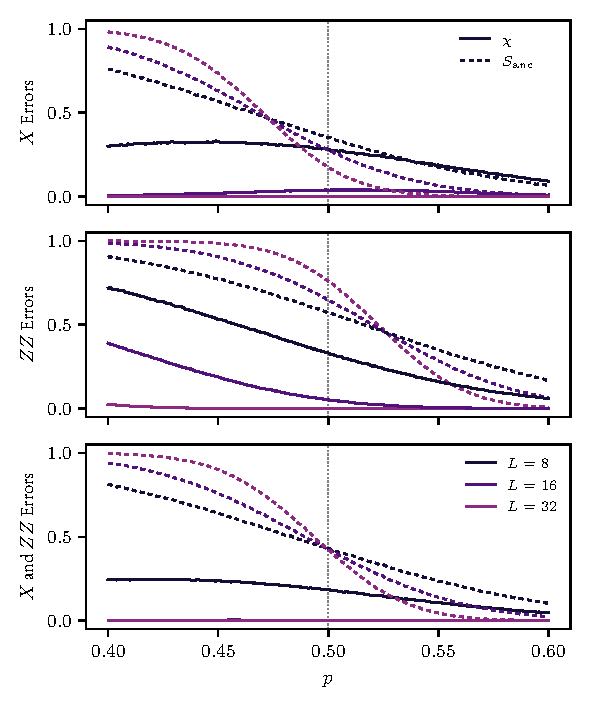
\includegraphics{anc_vs_lxe_new.pdf}
  \caption{Ancilla entanglement entropy and linear cross entropy for an error
  rate of $q=0.1$ to highlight the behavior of $S_\mathrm{anc}$. The system sizes are chosen smaller compared to
\cref{fig:err-vs-tra} since $\chi$ would be $0$ for larger systems. Note that
this is shown for the region around the critical point $p=.5$ in the ideal
case. This was done to make the shift of $S_\mathrm{anc}$ in $p$ more
noticeable without having the cross entropy be $0$ for ridiculously small
system sizes. Grey vertical dots indicate the critical point in the ideal case
of no errors.}
  \label{fig:large-q-anc-vs-lxe}
\end{figure}
what happens if we only track a subset of measurements?
\subsection{Marginalization}
\label{sec:lxe-err-subset}
Despite the fact that $\rho$ and $\sigma$ are being subjected to physically
different circuits, we can still separate the respective probabilities as we
did before. We just need to be careful with the interpretation. That is, we can
follow the derivation in \cref{eq:lxe-subset}, where we replace $C$ in the
probabilities conditioned on initial state $\rho$ with $\tilde{C}$:

\begin{align}
      \label{eq:lxe-subset-err}
      \chi_{\tilde{C},C} &= \sum_{\mathbf{m}} P(\mathbf{m} \mid \tilde{C}, \rho) \frac{P(\mathbf{m} \mid
      C, \sigma)}{\sum_{\mathbf{m}'}\left(P(\mathbf{m}' \mid
      C, \sigma)\right)^2} \nonumber\\
      \nonumber\\
      &= \sum_{\mathbf{m}_X \cap \mathbf{m}_Z} P(\mathbf{m}_X \cap \mathbf{m}_Z |
        \tilde{C}, \rho) \frac{P(\mathbf{m}_X \cap \mathbf{m}_Z| C,
        \sigma)}{\sum_{\mathbf{m}_X' \cap \mathbf{m}_Z'} \left(P(\mathbf{m}_X' \cap
        \mathbf{m}_Z'|C,\sigma)\right)^2}\nonumber\\
        \nonumber\\
      &= \sum_{\mathbf{m}_X \cap \mathbf{m}_Z} P(\mathbf{m}_X | \tilde{C}, \rho) P(
        \mathbf{m}_Z | \tilde{C}, \rho) \frac{P(\mathbf{m}_X | C, \sigma) P( \mathbf{m}_Z|
        C, \sigma)}{\sum_{\mathbf{m}_X' \cap \mathbf{m}_Z'}
          \left(P(\mathbf{m}_X' | C,
        \sigma) P( \mathbf{m}_Z'|C,\sigma)\right)^2}\nonumber\\
        \nonumber\\
      &= \underbrace{\frac{\sum_{\mathbf{m}_Z} P(\mathbf{m}_Z | \tilde{C}, \rho)
          P(\mathbf{m}_Z | C, \sigma)}{\sum_{\mathbf{m}_Z'}
          \left(P(\mathbf{m}_Z' |
          C, \sigma)\right)^2}}_{\text{Subset ZZ}}
          \underbrace{\frac{\sum_{\mathbf{m}_X} P(\mathbf{m}_X | \tilde{C}, \rho)
          P(\mathbf{m}_X | C, \sigma)}{\sum_{\mathbf{m}_X'}
          \left(P(\mathbf{m}_X' |
          C, \sigma)\right)^2}}_{\text{Subset X}}
\end{align}
It turns out that tracking $\mathcal{O}$ measurements only prevents us from
seeing $\mathcal{O}$-errors. It is not hard to convince oneself that this needs to
be true: If we do not care about the outcomes of the observable, where no errors
happen, then every error gets necessarily bypassed as described above. We can
no longer distinguish if a measurement turned from random to deterministic due
to a faulty random measurement. The outcome is still a valid one with respect to
$C$ (and possibly $\sigma$, for that matter). On the other hand will it be
impossible to tell if the entanglement cluster died because of a faulty
measurement or a native one. 

In particular will tracking only $X$ with $X$-errors be the same as without, which
is equivalent to tracking everything without errors. Furthermore will tracking
$ZZ$ while having $ZZ$ errors still be identically $1$. One can, of course,
combine the lot ad absurdum, which culminates into \cref{fig:err-vs-tra}, with
the quest of finding a worthy representative of the actual happenings inside
the PTIM.

\Cref{fig:err-vs-tra} shows multiple plots of $\chi$ as a function of
$p$, where $p$ ($1-p$) is the probability of a single-site $X$ ($ZZ$)
measurement. The plots are ordered as follows. In each row there is some kind of
error present: none, $X$, $ZZ$, and $X$ and $ZZ$. Each error happens at an
error rate of $q=0.01$. In each column, we track a different subset of
measurements, $X$, $ZZ$, and all measurements.
Inside the plots are annotations which qualitatively
indicate the mechanism behind $\chi$ going to $0$, refering to the previously
defined denotions of said mechanisms. The dashed line is the ancilla
entanglement entropy. Each simulation was done twice: once for an isolated
system, which we then compared with $\sigma$, and another one entangled to an
ancilla qubit. At the end of each circuit simulation, we computed the
entanglement entropy of the ancilla. It is $1$ if the cluster survived and $0$
otherwise. Its critical point should be lower for $X$ errors, higher for $ZZ$
errors and roughly equal to the ideal case for $X$ and $ZZ$ errors.
\Cref{fig:large-q-anc-vs-lxe} offers a visualization of this phenomenon.

\Cref{fig:err-vs-tra} hopefully looks nice. Maybe it also floats to the correct
place!
\begin{figure}[H]
  \centering
  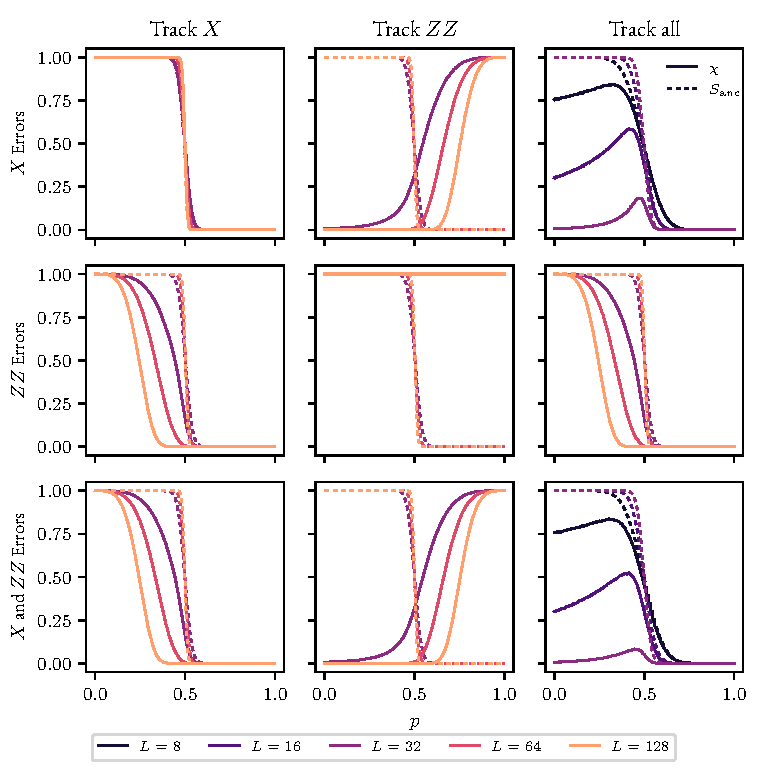
\includegraphics{errors-vs-tracked.pdf}
  \caption{Which measurement outcomes have been tracked and used to compute the
  linear cross entropy, vs the type of errors simulated.}
  \label{fig:err-vs-tra}
\end{figure}
%It didn't seem to do so, so i passed \texttt{[h!]}
\section{Summary}
